\documentclass[12pt,letterpaper]{article}
\usepackage[UTF8]{ctex}%Use Xelatex to compile
\usepackage{fullpage}
\usepackage[top=2cm, bottom=4.5cm, left=2.5cm, right=2.5cm]{geometry}
\usepackage{amsmath,amsthm,amsfonts,amssymb,amscd}
\usepackage{comment}
\usepackage{lastpage}
\usepackage{enumerate}
\usepackage{fancyhdr}
\usepackage{mathrsfs}
\usepackage{xcolor}
\usepackage{graphicx}
\usepackage{listings}
\usepackage{hyperref}
\usepackage{bm}
\usepackage{graphicx}

\hypersetup{%
  colorlinks=true,
  linkcolor=blue,
  linkbordercolor={0 0 1}
}


\usepackage{algorithm}
%\usepackage{algorithmicx}
%\usepackage{algorithmic}
\usepackage{algpseudocode}
\newenvironment{solution}{%
  \begin{proof}[Solution]$ $\par\nobreak\ignorespaces
}{%
  \end{proof}
}
\usepackage{enumitem}
\def \H{\mathcal H}
\def \z{\boldsymbol{z}}
\def \w{\boldsymbol{w}}
\def \x{\boldsymbol{x}}
\def \hint{\textbf{Hint: }}
\DeclareMathOperator*{\sign}{sign}
\DeclareMathOperator*{\WM}{Weighted Majority}
\DeclareMathOperator*{\E}{\mathbb{E}}


\lstdefinestyle{Python}{
    language        = Python,
    frame           = lines, 
    basicstyle      = \footnotesize,
    keywordstyle    = \color{blue},
    stringstyle     = \color{green},
    commentstyle    = \color{red}\ttfamily
}

\setlength{\parindent}{0.0in}
\setlength{\parskip}{0.05in}

%% Homework info.
\newcommand{\posted}{\text{Mar 14, 2022}}       			%%% FILL IN POST DATE HERE
\newcommand{\due}{\text{Apr 2 23:59, 2022}} 			%%% FILL IN Due DATE HERE
\newcommand{\hwno}{\text{2}} 		           			%%% FILL IN LECTURE NUMBER HERE


%%%%%%%%%%%%%%%%%%%%
%% Put your information here %%
%%%%%%%%%%%%%%%%%%%
\newcommand{\name}{\text{董浚哲}}  	          			%%% FILL IN YOUR NAME HERE
\newcommand{\id}{\text{2019011985}}		       			%%% FILL IN YOUR ID HERE
%%%%%%%%%%%%%%%%%%%%
%% End of the student's info %%
%%%%%%%%%%%%%%%%%%%


\lhead{
	\textbf{\name}
}
\rhead{
	\textbf{\id}
}
\chead{\textbf{
		Homework \hwno
}}


\begin{document}
\vspace*{-4\baselineskip}
\thispagestyle{empty}

\newcommand{\dd}{\,\mathrm{d}}
\newcommand{\R}{\mathbb{R}}
\newcommand{\st}{\text{ s.t. }}
\newcommand{\nm}[1]{\left\|#1\right\|}
\newcommand{\dual}[1]{\left<#1\right>}



\begin{center}
{\bf\large Mathematical Foundations of Machine Learning}\\
{Spring 2022}\\
Tsinghua University
\end{center}
\rule{\textwidth}{2pt}
\noindent
Lecturer: Yuan Zhou   			 %%% FILL IN LECTURER HERE
\hfill
\textbf{Homework \hwno}             			
\\
Posted: \posted
\hfill
Due: \due
\\
Name: \name             			
\hfill
ID: \id					
\hfill
\rule{\textwidth}{2pt}

\medskip
%\begin{center}
{ \it There are $10$ problems in this homework. The total amount of available points is 100. You may start to work on Problems 1--6 immediately. Problems 7--8 will be ready for you to work on after we finish Lecture 04. Problems 9--10 will be ready after we finish Lecture 05.}
%\end{center}


\begin{enumerate}
\item {[10 pts.]}
{\bf Tightness of Sauer's lemma.} For any set $C$ of $m > d$ elements, show that there exists a hypothesis class $\mathcal{H}$ of VC-dimension $d$ such that $\tau_{\mathcal{H}}(m)=\sum_{i=0}^{d}\binom{m}{i}$.
\begin{solution}
  Recall that we used the following inequalities to prove Sauer's lemma:
  \begin{enumerate}
  \item $\forall C=\{c_{1},\cdots,x_{m}\}$
    \[|H_{C}|\leq |\{B\subset C: H \text{ shatters } B\}|\]
    Take $\max$ at LHS and we get $\tau_{H}$
  \item \[|\{B\subset C: H \text{ shatters } B\}|\leq \sum_{i=0}^{d}\binom{m}{i}\]
  \end{enumerate}
  The second inequality is obviously tight, so it suffices to prove that the first is tight. As was done in lecture notes, we apply induction on $m$:
  \begin{itemize}
  \item \textbf{Step 1: } For $m=1$, both sizes are 2 if $C$ can be shattered.
  \item \textbf{Step 2: } Suppose the statement holds for $k<m$. Define $C'=\{c_{2},\cdots, c_{n}\}$, $Y_{0}=H_{C'}=\left\{\left(y_{2}, \ldots, y_{m}\right):\left(0, y_{2}, \ldots, y_{m}\right) \in \mathcal{H}_{C} \vee\left(1, y_{2}, \ldots, y_{m}\right) \in \mathcal{H}_{C}\right\}$, $Y_{1}=\left\{\left(y_{2}, \ldots, y_{m}\right):\left(0, y_{2}, \ldots, y_{m}\right) \in \mathcal{H}_{C} \land\left(1, y_{2}, \ldots, y_{m}\right) \in \mathcal{H}_{C}\right\}$.

    Here $|H_{C}|=|Y_{0}|+|Y_{1}|$
    
    By induction hypothesis, $|Y_{0}|=|H_{C'}|\leq |B\subset C': H \text{ shatters } B|=|\{B\subset C: c_{1}\not\in B\land H \text{ shatters }B\}|$ is tight. Denote the hypothesis class where the equation holds as $\tilde{H}$

    Define $\mathcal{H}^{\prime} =\left\{h \in \mathcal{H}: \exists h^{\prime} \in \mathcal{H} \text { s.t. }\left(1-h^{\prime}\left(c_{1}\right), h^{\prime}\left(c_{2}\right), \ldots, h^{\prime}\left(c_{m}\right)\right)\right.=\left(h\left(c_{1}\right), h\left(c_{2}\right), \ldots, h\left(c_{m}\right)\right\}$, then $|Y_{1}|=|H'_{C'}|\leq |\{B\subset C: c_{1}\in B\land H\text{ shatters } B\}|$, which by definition is tight. Denote the hypothesis class where the equation holds as $\tilde{H}'$.

    Take $H=\tilde H\cup \tilde H'$, and we see that $|H_{C}|=|Y_{0}|+|Y_{1}|=\leq \mid\left\{B \subseteq C: c_{1} \notin B \wedge \tilde{\mathcal{H}} \text { shatters } B\right\}|+|\left\{B \subseteq C: c_{1} \in B \wedge \tilde{\mathcal{H}} \text { shatters } B\right\} \mid 
=\mid\{B \subseteq C: \mathcal{H} \text { shatters } B\} \mid
\end{aligned}$
\end{itemize}

In conclusion, we've proved that Sauer's lemma is tight.
\end{solution}



\item {[10 pts.]} {\bf Tightness of the convergence theorem of the perceptron algorithm.} Show that for any positive integer $m$, there exist a vector $\bm{w}^{*} \in \mathbb{R}^{d}$ (for some appropriate $d$) and a sequence of examples $\left\{\left(\bm{x}_{1}, y_{1}\right), \ldots,\left(\bm{x}_{m}, y_{m}\right)\right\}$ such that the following hold:
\begin{itemize}
    \item  $R=\max _{i}\left\|\bm{x}_{i}\right\| \leq 1$.
    \item $\left\|\bm{w}^{*}\right\|^{2}=m$, and for all $i \leq m, y_{i}\left\langle\bm{x}_{i}, \bm{w}^{*}\right\rangle \geq 1$.
    \item When running the perceptron algorithm on this sequence of examples it makes $m$ updates before converging.
\end{itemize}


\begin{solution}
\begin{comment}
  If $\bm{w}$ and $\{(\bm x_{i},y_{i})\}_{i=1}^{m}$ satisfies these conditions, then in iteration $t\quad 1\leq t< m$:
  on one hand it was always wrong in previous examples, so
  \[\bm{w}^{(t)}=\sum_{i=1}^{t-1}y_{i}\bm{x}_{i}\]
  \[\bm{w}^{*}=\bm{w}^{(m)}=\sum_{i=1}^{m}y_{i}\bm{x}_{i}\]
  on the other hand, its guess is wrong in that iteration, so
  \[y_{t}\bm{x}_{t}^{T}\bm{w}^{(t)}\leq 0\]
  \[y_{t}\bm{x}_{t}^{T}\bm{w}^{*}\geq 1\]
  Merging the equations abve and we get:
  \[y_{t}\sum_{i=1}^{t-1}y_{i}\bm{x}_{i}^{T}\bm{x}_{t}\leq 0\]
  \[y_{t}\sum_{i=1}^{m}y_{i}\bm{x}_{i}^{T}\bm{x}_{t}\geq 1\]
  
  \begin{enumerate}[label=(\alph*)]
\item
\item
\item
\end{enumerate}
\end{comment}
  Suppose $\{(\x_{i},y_{i})\}_{i=1}^{m}$ is some set of training points. Run the perceptron algorithm, and we'll always get a corresbonding $\w^{*}$. At iteration $t$, by selecting appropriate $y_{(t)}$, $\w_{(t)}$ always has to be updated (so that (iii) is automatically satisfied). Also by lecture notes, at each update, $\w_{(t)}$ grows by at least $1$, so ot suffices to select $\x_{t}\st \w_{(t)}$ grows by no more than 1.

  Observe that
  \[\nm{\w_{(t+1)}}^{2}=\nm\{\w_{t}\}^{2}+2y_{t}\dual{\w_{t},\x_{t}}+\nm{x_{t}}^{2}\]
  So by selecting $\x_{t}\st \nm{x_{t}}=1,\dual{\w_{t},\x_{t}}$ (finding such a vector perpendicular to $\w_{t}$ is always possible as long as $d\geq 2$), then $\w_{t}$ grpws by exactly 1 at each iteration. In this way, (i)(ii) are satisfied.

\end{solution}

\item {[10 pts.]}  {\bf Small ball probabilities.} Let $X_{1}, \ldots, X_{N}$ be non-negative independent random variables with continuous distributions. Assume that the densities of $X_{i}$ are uniformly bounded by 1 .

\begin{enumerate}[label=(\alph*)]
    \item Show that the moment generating function of $X_{i}$ satisfies that $\mathrm{E} [\exp \left(-t X_{i}\right)] \leq \frac{1}{t}$ for all $t>0 .$
    
    \item Deduce that, for any $\varepsilon>0$, we have
$$
\Pr\left[\sum_{i=1}^{N} X_{i} \leq \varepsilon N\right] \leq(e \varepsilon)^{N} .
$$
\end{enumerate}

\begin{solution}
\begin{enumerate}[label=(\alph*)]
\item Denote the p.d.f of $X_{i}$ as $f_{i}(w)$, where by assumption $f_{i}(w)\leq 1$. Then by definition $E[\exp(-tX_{i})]=\int_{\R_{+}}e^{-tw}f(w)\dd w\leq \int_{0}^{\infty}e^{-tw}\dd w=\frac{1}{t}$
\item Since $\varepsilon>0$,$P[\sum_{i=1}^{N}X_{n}\leq \varepsilon N]=P[-\sum_{i=1}^{N}\frac{1}{\varepsilon}X_{i}\geq -N]=P[\exp(\sum_{i=1}^{n}-\frac{1}{\varepsilon}X_{i})\geq e^{-N}]\leq e^{N}\prod_{i=1}^{N}E[\exp(-\frac{1}{\varepsilon}X_{i})]$. So by (a), $P[\sum_{i=1}^{N}X_{i}\leq\varepsilon N]\leq (e\varepsilon)^{N}$
\end{enumerate}
\end{solution}


\item {[10 pts.]}
{\bf Robust estimation of the mean.} Suppose we want to  estimate the mean $\mu$ of a random variable $X$ from the samples $X_{1}, \ldots, X_{N}$ drawn independently from the its distribution. We want an $\varepsilon$-accurate estimate, i.e.~one that falls in the interval $(\mu-\varepsilon, \mu+\varepsilon)$.
\begin{enumerate}[label=(\alph*)]
    \item Show that a sample of size $N=O\left(\sigma^{2} / \varepsilon^{2}\right)$ is sufficient to find an $\varepsilon$-accurate estimate with probability at least $3 / 4$, where $\sigma^{2}=\operatorname{Var}[X]$.
    \item Show that a sample of size $N=O\left(\log \left(\delta^{-1}\right) \sigma^{2} / \varepsilon^{2}\right)$ is sufficient to find an $\varepsilon$-accurate estimate with probability at least $1-\delta$.
\end{enumerate}
(\textbf{Hint:} Note that in this exercise we do not assume any bounds for the support of $X$.)
\begin{solution}
  (a) is a direct corrolary of (b), so it suffices to prove (b).
  
  WLOG assume $\mu=0$, otherwise replace $X_{i}$ with $X_{i}-\mu$

  $P(-\varepsilon<\frac{1}{N}\sum_{i=1}^{N}X_{i}<\varepsilon)=P(\sum_{i=1}^{N}X_{i}^{2}\leq N^{2}\varepsilon^{2})$. By Markov's inequality, $P(\sum_{i=1}^{N}X_{i}^{2}\geq N^{2}\varepsilon^{2})\leq \frac{E[\sum_{i=1}^{N}X_{i}^{2}]}{N^{2}\varepsilon^{2}}$. Since $E[\sum_{i=1}^{n}X_{i}^{2}]=\sum_{i=1}^{N}E[X_{i}^{2}]=N\sigma^{2}$, so $P(\sum_{i=1}^{N}X_{i}^{2}\geq N^{2}\varepsilon^{2})\leq \frac{\sigma^{2}}{N\varepsilon^{2}}$. bring in the estimate of $N$ and we get $P(|\frac{1}{N}\sum_{i=1}^{N}X_{i}|<\varepsilon)=1-P(\sum_{i=1}^{N}X_{i}^{2}\geq N^{2}\varepsilon^{2})\geq 1-\delta$, thus we get the desired estimate.

\end{solution}

\item {[10 pts.]} {\bf Hoeffding's lemma via symmetrization.}
In class (Lecture 03) we stated the following Hoeffding's lemma without a proof: if $X$ is zero-mean and has support $X \in [a, b]$, then $X$ is sub-Gaussian with parameter $\sigma=(b-a)/2$. In this exercise, we will derive an elegant proof of a slightly worse bound via the symmetrization trick.

\begin{enumerate}[label=(\alph*)]
\item Prove that the Rademacher random variable (i.e.~the random variable $\tau$ such that $\tau=1$ with probability $1/2$ and $\tau=-1$ with probability $1/2$) is sub-Gaussian with parameter $\sigma=1$.
\item The two samples trick: prove that $ \E_{X}\left[e^{\lambda X}\right] \leq \E_{X, X^{\prime}}\left[e^{\lambda\left(X-X^{\prime}\right)}\right] $, where $X'$ is an extra independent copy of $X$.
\item The symmetrization trick: prove that $ \E_{X, X^{\prime}}\left[e^{\lambda\left(X-X^{\prime}\right)}\right] \leq e^{\frac{\lambda^2(b-a)^2}{2}} $. Thus, $X$ is sub-Gaussian with parameter $(b-a)$.
\end{enumerate}

\begin{solution}
\begin{enumerate}[label=(\alph*)]
\item
  Claim: $\forall\lambda\in\R, e^{\lambda^{2}}-\frac{e^{\lambda}+e^{-\lambda}}{2}>0$. This is approved by Wolfram Alpha:

  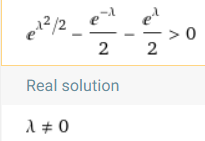
\includegraphics[scale=0.5]{pic.png}
  
  $\exp(\lambda\tau)=
  \begin{cases}
    e^{-\lambda}& \tau=-1\\ e^{\lambda}&\tau=1
  \end{cases}
  $.
  So $E[\exp(\lambda\tau)]=\frac{e^{-\lambda}+e^{\lambda}}{2}\leq \exp(\frac{1^{2}\cdot \lambda^{2}}{2})$
\item
  $E_{X,X'}[e^{\lambda(X-X')}]=\iint_{\Omega\times \Omega}e^{-\lambda(X-X')}\dd P\dd P=\int_{\Omega}e^{-\lambda X'}E[e^{\lambda X}]\dd P=E[e^{\lambda X}]E[e^{-\lambda X}]$. Observe that $E[X]=0$ and that $e^{-\lambda X}\geq 1+\lambda X$, take expectation on both sides and we get $E[e^{-\lambda X}]\geq 1$, so $E_{X}[e^{\lambda X}]\leq E_{X,X'}[e^{\lambda(X-X')}]$
\item In the worst case, $X,X'$ only takes values on the boundaries and worse still, $X-X'$ only takes values on the boundary ($X-X'\neq 0\quad a.e.$), then $P(X-X'=b-a)=P(X-X'=-(b-a))=\frac{1}{2}$, in which case $\frac{X-X'}{b-a}$ is Rademacher r.v. $\Rightarrow \frac{X-X'}{b-a}$ is sub-gaussian with variance proxy $1\Rightarrow X-X'$ is sub-Gaussian with variance proxy $(b-a)$. The proposition follows from the definition. 

\end{enumerate}
\end{solution}

\item {[10 pts.]} {\bf Tightness of the Chernoff Bounds.}
\begin{enumerate}[label=(\alph*)]
    \item  Show that the Chernoff Bounds are asymptotically tight. More concretely, prove the following statement: For any $\mu \in[0,1 / 2]$ and $\delta \in(0,1)$, show that there exist infinitely many $n \in \mathbb{N}$, a sequence of $n$ independent random variables $\left\{X_{i}\right\}_{i=1}^{n}$ such that $X_{i} \in[0,1]$ almost surely, $\E\left[X_{i}\right]=\mu$, and
$$
\Pr\left[\sum_{i=1}^{n} X_{i} \geq(1+\delta) n \mu\right] \geq \exp (-O(\delta^{2} n \mu))
$$
    \item Let $\mathcal{D}$ be a distribution supported on $[0,1]$. Let $\mu(\mathcal{D})=\E_{X \sim \mathcal{D}}[X] .$ Let $X_{1}, X_{2}, \ldots, X_{n}$ be \emph{i.i.d.}~drawn from $\mathcal{D}$. Define
$$
g(n, \mathcal{D}) \stackrel{\text { def }}{=} \Pr\left[\sum_{i=1}^{n} X_{i} \geq n \sqrt{\mu(\mathcal{D})}\right] 
$$
Find a function $f(\mu)$ such that for all $\mu \in(0, \mu_{0})$ there exists a positive integer $N=N(\mu)$ when $n>N$, it holds that
$$
\exp (-C n \cdot f(\mu)) \leq \sup _{\mathcal{D}: \mu(\mathcal{D})=\mu} g(n, \mathcal{D}) \leq \exp (-c n \cdot f(\mu)),
$$
where $c, C, \mu_{0}$ are universal constants.
\end{enumerate}
\begin{solution}
\begin{enumerate}[label=(\alph*)]
\item
  $e^{-\delta^{2}n\mu}=((e^{\delta n\mu}-1)+1)^{-\delta}\approx (1+\delta)-\delta e^{n\delta \mu}$

  $I=P[\sum_{i=1}^{N}X_{i}\geq (1+\delta)n\mu]=1-P[\exp(-\sum_{i=1}^{N}X_{i})>\exp(-(1+\delta)n\mu)]$. By Markov's inequality, $I\geq 1-e^{(1+\delta)n\mu}\prod_{i=1}^{n}E[\exp(-X_{i})]$. So it suffices to choose $X_{i}\st E[e^{-X_{i}}]\geq \delta^{\frac 1 n}e^{-\mu}$. This is generally possible as long as $n$ is big enough $\st \delta^{\frac 1 n}\approx 1$ and an appropriate Bernoulli distribution $X\sim\frac{1}{m}B(\mu,m) $ always satisfies these properties.
\item %Apply Chernoff's method and we have $g(n,\mathcal{D})\leq e^{-n\sqrt{\mu}}\prod_{i=1}^{n}\mu$

  I don't understand......
\end{enumerate}
\end{solution}

\item {[10 pts.]} {\bf Least squares for general $X$.} When discussing the least squares method in Lecture 04, we showed that when $X$ is such that $XX^\top$ is invertible, $\bm{w} = (XX^\top)^{-1} X\bm{y}$ is the solution to 
\begin{align}
 X (X^\top \bm{w} - \bm{y}) = \bm{0}. \label{eq:prob-6}
\end{align}
For general $X$, we will derive a closed-form solution to Eq.~(\ref{eq:prob-6}) in this exercise. For this purpose, we first need to define the pseudo-inverse of and real matrix $A \in \mathbb{R}^{m\times n}$ as follows. We write out the (compact) singular value decomposition of $A$ as below,
\[
A = U D V^\top
\]
where $U$ and $V$ are orthonormal matrices and $D\in \mathbb{R}^{m \times n}$ is a rectangular diagonal matrix  with non-negative entries (i.e., the only non-zero entries are at $d_{ii} \geq 0$ where $i \in \{1, 2, \dots, \min\{n, m\}\}$). The elements in the diagonal entries of $D$ are the \emph{singular values} of $X$.

Now we define the \emph{pseudo-inverse} (a.k.a.~the \emph{Moore–Penrose inverse}) of $A$ to be 
\[
A^+ = V D^{+} U^\top,
\]
where $D^+$ is replacing every non-zero element in $D$ by its scalar inverse.

Now, please show that $\bm{w} = (X^+)^\top \bm{y} = (XX^\top)^+ X\bm{y}$ satisfies Eq.~(\ref{eq:prob-6}).

\begin{solution}
  First we reduce Eq.\ref{eq:prob-6} with SVD: assume $X$ has the SVD decomposition $X=UDV^{T}$, then $XX^{T}=UD^{2}U^{T}$, so the equation reduces to
  \[D^{2}U^{T}\bm{w}-DV^{T}\bm{y}=\bm{0}\]

  Secondly, we'll prove $(X^{+})^{T}=(XX^{T})X$ so that we only need to verify the case where $\bm{w}=(X^{+})^{T}\bm{y}$. $(XX^{T})^{+}=U(D^{+})^{2}U\Rightarrow (XX^{T})^{+}X=UD^{+}D^{+}UUDV^{T}=UD^{+}V^{T}=(VD^{+}U)^{T}=(X^{+})^{T}$

  Finally, we take $\bm{w}=(X^{+})^{T}y$ into LHS and get $D^{2}U^{T}UD^{+}V^{T}y-DV^{T}y=0=RHS$. Thus we've verified the equation.
\end{solution}

\item {[10 pts.]} {\bf Failure of the $k$-fold cross validation.} Consider a case in that the label is chosen at random according to $\Pr[y = 1] = \Pr[y = 0] = 1/2$. Consider a learning algorithm that outputs the constant predictor $h(x) = 1$ if the parity of the labels on the training set is $1$ and otherwise the algorithm outputs the constant predictor $h(x) = 0$. Prove that the difference between the leave-one-out estimate (LOO estimate, a special case of the $k$-fold cross validation where $k$ equals to $m$, the number of available samples) and the true error in such a case is always $1/2$.
\begin{solution}
  Denote the samples as $\{(x_{i},y_{i})_{i=1}^{m}\}$, where half of $y_{i}=0$. At iteration $t$, if $y_{t}=0$, then $h(x)=1$; if $y_{t}=1$, then $h(x)=0$. In both cases, the validation error is always $1$ while the true error is always $\frac{1}{2}$. The statement thus follows.  
\end{solution}

\item {[10 pts.]} {\bf Completing the proof in Lecture 05.} In the slide ``Connection to Chernoff/Hoeffding Bounds'' of Lecture 05, we stated a claim and left it as an exercise. Please prove this claim: for any iteration $t$, we have that 
\[
\epsilon_t = \sum_{\bm{x} \in \mathcal{X}} D_{\bm{x}}^{(t)} \mathbf{1}[h_t(\bm{x}) = +1] = \frac12 - \gamma .
\]

\begin{solution}
  $D_{\x}^{(1)}=\prod_{i=1}^{n}[(\frac{1}{2}+\gamma)^{\frac{1+x_{i}}{2}}(\frac{1}{2}-\gamma)^{\frac{1-x_{i}}{2}}]$. By definition, $\varepsilon_{t}=\sum_{\bm{x}:x_{t}=-1}D_{\bm{x}}^{(t)}$.

  We prove by inducution on $t$. %Here we denote $w=\frac{1}{2}\log(\frac{1/2+\gamma}{1/2-\gamma})$.

  \textbf{Step 1:} For $t=1$, $\varepsilon_{1}=\sum_{\bm{x}:x_{1}=-1}D^{(1)}_{\x}=(frac{1}{2}-\gamma)\sum_{\tilde{\x}\in\{\pm 1\}^{n-1}}\prod_{i=2}^{n}[(\frac{1}{2}+\gamma)(\frac{1}{2}-\gamma)]$. On this last equation we use induction on $n$: $n=1$ is the trivial case. Suppose the equation is true for $n=k$, then for $n=k+1$, $ \sum_{\bm{x}\in\{\pm 1\}^{k+1}}[(\frac{1}{2}+\gamma)(\frac{1}{2}-\gamma)]=(\frac{1}{2}+\gamma)\sum_{\bm{x}\in\{\pm 1\}^{k}}[(\frac{1}{2}+\gamma)(\frac{1}{2}-\gamma)]+(\frac{1}{2}-\gamma)\sum_{\bm{x}\in\{\pm 1\}^{k+1}}[(\frac{1}{2}+\gamma)(\frac{1}{2}-\gamma)]=1$.

  \textbf{Step 2:} Suppose the statement is true for $t\leq k$, then for $t=k+1$, $\varepsilon_{k+1}=\sum_{\bm{x}:x_{k+1}=-1}D^{(k+1)}_{\x}=\frac{1}{Z_{k}}\sum_{\x: x_{k+1}=-1,x_{k}=1}D_{\x}^{(k)}D_{\x}^{(t)}\sqrt{\frac{1/2+\gamma}{1/2-\gamma}}+\frac{1}{Z_{k}}\sum_{\x:x_{k+1}=-1,x_{k}=-1}\sqrt{\frac{1/2-\gamma}{1/2+\gamma}}$. Also by trivial inductio we see that $Z_{t}=\frac{1}{2}(\sqrt{\frac{1/2+\gamma}{1/2-\gamma}}+\sqrt{\frac{1/2-\gamma}{1/2+\gamma}})$, so by induction hypothesis $\varepsilon_{(k+1)}=2(\frac{1}{2}-\gamma)\cdot\frac{1}{2}=\frac{1}{2}-\gamma$. The last $\frac{1}{2}$ comes from the fact that exactly half of the sample points with the same distribution w.r.t. first $k$ coordinates are in the sum.
\end{solution}

\item {[10 pts.]} Let $\mathcal{X}_{n}=\{0,1\}$, and let $\mathcal{G}_{n}$ be a class of Boolean functions $ g: \mathcal{X}_{n} \rightarrow\{-1,+1\}$. Let $\mathcal{M}_{n, k}$  be the class of all Boolean functions that can be written as a simple majority vote of $k$ (not necessarily distinct) functions in $\mathcal G_{n}$, where $k$ is odd:
$$
\mathcal{M}_{n, k} \doteq\left\{f: x \mapsto \operatorname{sign}\left(\sum_{j=1}^{k} g_{j}(x)\right) \mid g_{1}, \ldots, g_{k} \in \mathcal{G}_{n}\right\}
$$
In this problem we will see, roughly speaking, that if $f$ can be written as a majority vote of polynomially many functions in $\mathcal G_{n}$, then under any distribution, $f$ can be approximated by some function in $\mathcal G_{n}$. But if $f$ cannot be so written as a majority vote, then there exists some ``hard'' distribution under which $f$ cannot be approximated by any $\mathcal{G}_{n}$.
\begin{enumerate}[label=(\alph*)]
    \item  Show that if $f \in \mathcal{M}_{n, k}$, then for every distribution $D$ on $\mathcal{X}_{n}$, there exists a function $ g \in G_{n}$ for which
\[
\Pr_{x \sim D}[f(x) \neq g(x)] \leq \frac{1}{2}-\frac{1}{2 k} .
\]
    \item Show that if $f \notin \mathcal{M}_{n, k}$, then there exists a distribution $D$ on $\mathcal{X}_{n}$ such that 
\[
\Pr_{x \sim D}[f(x) \neq g(x)]>\frac{1}{2}-\sqrt{\frac{n \ln 2}{2 k}}
\]
for every $g \in \mathcal{G}_{n}$.
\end{enumerate}
(\hint Use Boosting.)



\end{enumerate}
\begin{solution}
\begin{enumerate}[label=(\alph*)]
\item Suppose $f(x)=\mathrm{sign}(\sum_{j=1}^{k}g_{j}(x))$. Apply adaptive boosting with $T=k, h_{j}=g_{j}$, thenwe get $g=\mathrm{sign}(\sum_{j=1}^{k}w_{j}g_{j}(x))\in G_{n}$.

  At iteration $t$, $\varepsilon_{t}=\sum_{\x\sim\mathcal{D}}D^{(t)}_{\x}\bm{1}_{A_{t}}$, where $A_{t}=\{f(\x)\neq g_{t}(\x)\}=\{\mathrm{sign}(\sum_{j=1}^{k}g_{j}(\x))\neq g_{t}(\x)\}$. So $\forall\x\sim D$, $D_{\x}^{(t)}$ is increasedby no more than $\frac{k-1}{2}$ times while decreased by no less than $\frac{k+1}{2}$ times. So the worst case is equivalant to the case of doing 1 iteration on the desired points, which results in the error $P[f(x)\neq g(x)]=\frac{1}{k}(\frac{k-1}{2})=\frac{1}{2}-\frac{1}{2k}$
\item
   I don't really understand......
  
\end{enumerate}
\end{solution}


\end{document}

%%% Local Variables:
%%% mode: latex
%%% TeX-master: t
%%% End:
